\chapter{Implementação}

\section{Autômato celular}

\subsection{Modelo inicial}

O autômato celular inicialmente proposto possui 24 estados discretos. Esses estados correspondem aos 20 aminoácidos, aos 3 elementos de estruturas secundárias (hélice, fita e random coil) e mais um estado que indica o início/fim da cadeia polipeptídica (\textit{estado=\#}). A vizinhança deste autômato celular é igual a 1 (\textit{r}=1),  o que indica que as regras de transição são dependentes dos dois vizinhos mais próximos, um a esquerda e um a direita. Cada transição pode ocorrer para apenas quatro estados, send 3 estados que representam os elementos de estrutura secundária e um que representa o resíduo presente naquela posição da cadeia polipeptídica.

Logo, temos que o total de elementos na regra desse autômato é $24^3$ ou 13824, doss quais 24 são elementos estáticos, pois células no estado \textit{\#} sempre permanecerão nesse estado durante a evolução do autômato. Assim temos $4^{24^3-24}$ regras possíveis para esse autômato celular.

\begin{figure}
  \centering
  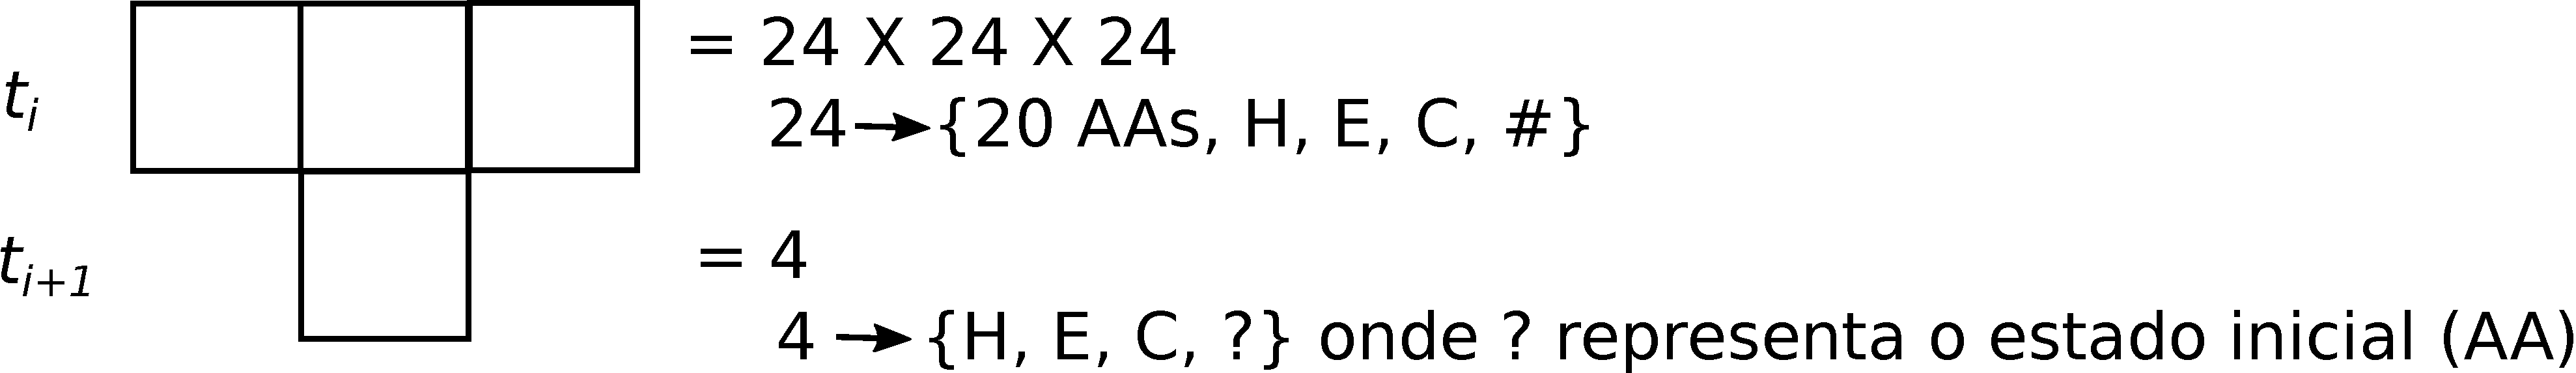
\includegraphics[width=.8\textwidth]{figures/ca_rule_scheme.pdf}
  \caption{Esquema da regra simples}
        \label{fig:ca_rule_scheme}
\end{figure}

\subsection{Modelos extendidos}

Uma das limitações do modelo proposto inicialmente é a perda de informação que ocorre durante a evolução do autômato celular quando as células transitam de estados correpondentes aos aminoácidos para estados que representam elementos de estruturas secundárias. Por exemplo, quando uma lisina evolui para uma hélice, o estado de hélice não possui mais a informação de qual aminoácido havia naquela posição. Acreditamos que essa perda de informação possa ser um fator crítico para o modelo. Consequentemente, avaliamos modelos alternativos que pudessem manter essa informação. 

Uma possibilidade seria manter a informação do resíduo juntamente com o elemento de estrutura secundária. Esse modelo teria 20 estados para os aminoácidos, 20 estados para hélices (um estado diferente para cada aminoácido), 20 estados para fitas e 20 estados para random coils, além do estado de início/fim da cadeia polipeptídica, totalizando 81 estados. Cada regra para esse autômato celular teria $81^3$  ou 531441 elementos, o que seria aproximadamente 38 vezes maior que uma regra do modelo proposto inicialmente, resultando em um aumento significativo da complexidade e, consequentemente, da dificuldade na busca por regras que reproduzam o padrão desejado. Esse aumento de complexidade nos levou a descartar, pelo menos até o momento, este modelo.

Assim, a alternativa escolhida foi utilizar características dos aminoácidos que mantivessem parcialmente a informação do resíduo durante a evolução do autômato celular, mas sem resultar em um aumento tão elevado do número de regras em relação ao modelo inicial. O primeiro modelo concebido que atende esses requisitos utiliza as características de hidrofobicidade dos aminoácidos. Isso resulta em modelo com 27 estados, sendo 2 estados para cada um dos 3 elementos de estrutura secundária, mais os 20 aminoácidos e o início/fim da cadeia polipeptídica. No total, a regra deste autômato celular é formada por  $27^3$, ou 19683, elementos, sendo aproximadamente 1,42 vezes maior que a regra do modelo inicial.

Além deste modelo extendido, dois outros modelos foram utilizados. Um deles adicionando estados para diferenciar glicinas e prolinas, e outro acrescentando estados para diferencia resíduos com cargas positivas e negativas assim como glicinas e prolinas. Ambos utilizam também a hidrofobicidade dos demais resíduos. As regras para esses modelos apresentam  respectivamente $33^3$ e $39^3$ elementos, o que corresponde a um aumento aproximado de 2,6 e 4,3 vezes em relação ao modelo inicial. 

A motivação para o uso da hidrofobicidade dos resíduos foi influenciada por trabalhos de Hecht e colaboradores \cite{Xiong07, West1995} que examinaram a influência de padrões periódicos de hidrofobicidade nas sequências proteicas e sua relação com elementos de estruturas secundárias, concluindo que alguns padrões apresentam preferência por hélices $\alpha$ enquanto outros padrões apresentam preferência por fitas $\beta$ \cite{West1995}.

Em todos os modelos extendidos cada elemento da regra continua com a possibilidade de transitar para apenas 4 estados, ou um dos 3 elementos de estrutura secundária ou o resíduo encontrado naquela posição da cadeia polipeptídica.

\section{EDA}

A busca por regras de um autômato celular que reproduzam um padrão específico, conhecido como problema inverso, é um problema de otimização. Na literatura, esse problema é normalmente abordado utilizando metaheurísticas como algoritmos genéticos ou anelamento simulado (\textit{simulated annealing}). Neste trabalho optamos por utilizar o Algoritmo de Estimação de Distribuição (EDA). Os fatores que determinaram a utilização desse algoritmo foram a facilidade de implementação do EDA de forma distribuída e o pequeno número de parâmetros em relação à algoritmos genéticos.

No EDA distribuído implementado neste trabalho cada elemento da regra do autômato celular, com excessão dos elementos onde a célula apresenta o estado início/fim da cadeia polipeptídica (\textit{estado=\#}),  tem a mesma probabilidade inicial ($p=0,25$) para cada um dos 4 estados de transição. A probabilidade é distribuída pelo nó mestre para os nós escravos. Os nós escravos utilizam a probabilidade recebida para gerar $c \ge 2 $ regras candidatas. As regras candidatas são então utilizadas para evoluir o autômato celular por $t$ passos. Após a evolução, um valor de fitness é atribuído a cada regra. Em seguida, um torneio entre as regras candidatas geradas no nó escravo e a regra com maior fitness é enviada ao nó mestre. Ao recever as $n/c$ regras vencedoras, onde $n$ é o tamanho da população do EDA, o nó mestre atualiza a probabilidade e começa a distribuí-la para os nós escravos, iniciando assim a geração $T+1$ do EDA. A otimização termina após um número específicos de gerações ou quando as probabilidades convergem.

\subsection{Função de fitness}

A função de fitness utilizada pelo EDA baseia-se na porcentagem de estados corretos durante a evolução do autômato celular ($t_1 \rightarrow t_{final}$) onde os estados corretos são os elementos de estrutura secundária idênticos ao concenso obtido entre os quatro métodos de atribuição de estruturas secundária. Quando não há concenso entre os métodos de atribuição de estrutura secundária, a posição é descartada pela função de fitness. A função de fitness é, portanto, equivalente a acurácia.

\begin{equation}
ACC = \frac{TP + TN}{P + N}
\end{equation}
\begin{equation}
fitness =  \frac{TH + TE + TC}{H + E + C}
\end{equation}

\section{Implementação}

Tanto o autômato celular quanto o EDA foram implementados na linguagem de programação Go. A estrada do nó mestre é um arquivo de configuração no formato TOML que contém os parâmetros para o autômato celular, o EDA e os dados a serem utilizados. Os dados, ou seja as sequências de aminoácidos das proteínas e suas respectivas estruturas secundárias, são armazenados em um banco de dados chave/valor. A comunicação entre os nós escravo e o nó mestre é feita utilizando chamadas remotas de procedimento (RPC). O código fonte está acessível publicamente no GitHub (\href{https://github.com/jgcarvalho/zeca-search}{github.com/jgcarvalho/zeca-search}, \href{https://github.com/jgcarvalho/zeca-search-master}{zeca-search-master} e \href{https://github.com/jgcarvalho/zeca-search-slave}{zeca-search-slave})  

